\documentclass[journal]{IEEEtran}

\usepackage[utf8]{inputenc}
\usepackage[T1]{fontenc}
\usepackage[spanish,es-tabla,es-nodecimaldot]{babel}
\usepackage{amsmath,amssymb}
\usepackage{graphicx}
\usepackage{booktabs}
\usepackage{tabularx}
\usepackage{array}
\usepackage{siunitx}
\usepackage[hidelinks]{hyperref}

\sisetup{output-decimal-marker={,}, group-separator={\,}, group-minimum-digits=4}
\graphicspath{{figuras/}}

\begin{document}

\title{Factores asociados a la insatisfacción de clientes en el comercio electrónico: un enfoque de aprendizaje de máquina sobre los datos de Olist}

\author{Jaime~Alexis~Herrera, Julián~Andrés~Rodríguez y Camilo~Marsel~Cespedes%
\thanks{Modelos y Simulación II, Departamento de Ingeniería de Sistemas, Universidad de Antioquia.}}

\markboth{Modelos y Simulación II, Universidad de Antioquia, 2026}{}

\maketitle

\iffalse
\begin{abstract}
Olist es un marketplace brasileño que conecta pequeños y medianos comerciantes con los principales portales de comercio electrónico. Después de cada compra, el cliente califica su experiencia de 1 a 5; una calificación baja deteriora la reputación del vendedor y la confianza en la plataforma. Planteamos un clasificador binario para anticipar si una orden entregada recibirá una calificación de 1 o 2 a partir de variables de la orden, el producto, el pago y la entrega. Al analizar \num{95824} órdenes entregadas entre 2016 y 2018, con un 12,8~\% de clientes insatisfechos, el análisis exploratorio confirma que el retraso frente a la fecha prometida es el factor más asociado: la insatisfacción pasa de 9,2~\% en órdenes a tiempo a 54,1~\% en órdenes tardías.
\end{abstract}

\begin{IEEEkeywords}
Comercio electrónico, satisfacción del cliente, clasificación desbalanceada, aprendizaje supervisado, Olist.
\end{IEEEkeywords}
\fi


\section{Descripción del problema}

\IEEEPARstart{E}{n} el ecosistema actual del comercio electrónico, la fidelización del cliente es un factor de vital importancia para el crecimiento y la obtención de ganancias por parte de estas plataformas. Olist, una de las mayores aplicaciones de comercio electrónico en Brasil que conecta a pequeñas y medianas empresas con consumidores en todo el país, se enfrenta a un desafío que es propio a su modelo de negocio a gran escala: la gestión de la experiencia del cliente frente a una alta variabilidad operativa y logística. A pesar del éxito en las ventas y la gran acogida por la comunidad, una proporción significativa de los clientes experimentan altos niveles de insatisfacción, reflejados en calificaciones bajas respecto al servicio prestado por la plataforma. Como se evidenció en la exploración preliminar, aproximadamente el 14.7\% de las órdenes presentan este nivel de rechazo, principalmente asociado a deficiencias logísticas como tiempos de entrega prolongados y discrepancias entre la fecha estimada y la fecha real de llegada del producto.

Este indicador no solo representa un cliente insatisfecho, sino que impacta directamente en las métricas de retención, incrementando la tasa de abandono y afectando la reputación de la marca frente a nuevos compradores. Tradicionalmente, la gestión de la insatisfacción en el comercio electrónico (y en michos otros sectores del comercio) se basa en un proceso reactivo: la empresa interviene únicamente después de que el usuario ha dejado una reseña negativa o ha radicado una queja (PQRS), momento en el cual la relación comercial con el cliente ya está afectada y el riesgo de pérdida es demasiado alta.

El desarrollo de una solución basada en técnicas de Aprendizaje de Máquina (ML) resulta fundamental y altamente útil para transformar este enfoque reactivo en uno predictivo y proactivo que entregaría información útil a las empresas y plataformas digitales como Olist. Mediante el entrenamiento de algoritmos de clasificación supervisada, es posible identificar de manera anticipada patrones y relaciones entre las variables operativas (tiempos logísticos, valor del flete, cantidad de vendedores involucrados, métodos de pago y ubicación geográfica) para predecir la probabilidad de que una orden resulte en una experiencia insatisfactoria para el cliente. 


\subsection{Base de datos}

Para este proyecto utilizamos el \emph{Brazilian E-Commerce Public Dataset} proporcionado por Olist en la plataforma de kaggle~\cite{olist2018}. Originalmente, la base de datos está dividida en 9 tablas relacionales que contienen información sobre órdenes, clientes, productos, vendedores, reseñas y pagos (Tabla~\ref{tab:tablas}).

\begin{table}[h!]
\centering
\caption{Tablas originales del conjunto de datos}
\label{tab:tablas}
\begin{tabular}{@{}lrrl@{}}
\toprule
Tabla & Filas & Col. & Contenido \\
\midrule
orders & \num{99441} & 8 & estado y fechas de la orden \\
order\_items & \num{112650} & 7 & artículos, precio, flete \\
order\_payments & \num{103886} & 5 & tipo, cuotas y valor del pago \\
order\_reviews & \num{99224} & 7 & calificación y comentario \\
products & \num{32951} & 9 & categoría, peso, dimensiones \\
customers & \num{99441} & 5 & código postal y estado \\
sellers & \num{3095} & 4 & código postal y estado \\
geolocation & \num{1000163} & 5 & coordenadas por código postal \\
category\_translation & 71 & 2 & nombre de categoría en inglés \\
\bottomrule
\end{tabular}
\end{table}

\subsubsection{Número de muestras y unidad de análisis}
Decidimos que nuestra unidad de análisis principal sea el pedido individual (orden de compra). Al cruzar la información de las diferentes tablas y filtrar únicamente las órdenes que tienen un estado de ``entregado'' (delivered), que cuentan con una fecha real de entrega y que recibieron una reseña por parte del cliente, logramos consolidar una base de datos final de 95.824 muestras (órdenes) correspondientes a 92.747 clientes.

\vspace{1.5em}
\subsubsection{Número de variables y su significado}
Tras el cruce de tablas, construimos un total de 30 variables de entrada por cada orden, agrupadas de la siguiente manera:

\begin{itemize}
    \item Variables Logísticas y de Tiempo (Numéricas continuas y Binarias): Incluyen los días transcurridos desde la compra hasta la entrega, los días de retraso frente a la fecha prometida, el tiempo que tardó el vendedor en entregar a la transportadora, y dos variables binarias (0/1) que indican si el pedido en general llegó tarde y si el vendedor despachó tarde.
    \item Variables Económicas y de Pago (Numéricas continuas y Discretas): Incluyen el precio total de los artículos, el costo total del flete, la proporción del costo del flete sobre el precio del producto, el valor total pagado por el cliente y el número de cuotas seleccionadas.
    \item Variables del Producto y Geográficas (Numéricas y Categóricas): Contienen el número de artículos por pedido, peso y volumen de los productos, cantidad de fotos en la publicación. También se calculó la distancia en kilómetros entre el vendedor y el comprador usando las coordenadas, y se incluyeron los estados geográficos de origen y destino.
    \item Variable Objetivo (Binaria): Clasificamos a los clientes en ``Satisfechos'' (clase 0) si calificaron con 3, 4 o 5 estrellas, e ``Insatisfechos'' (clase 1) si calificaron con 1 o 2 estrellas. Bajo esta regla, el 12.8\% de nuestras órdenes corresponden a clientes insatisfechos (Fig.~\ref{fig:score}).
\end{itemize}


\begin{figure}[h!]
\centering
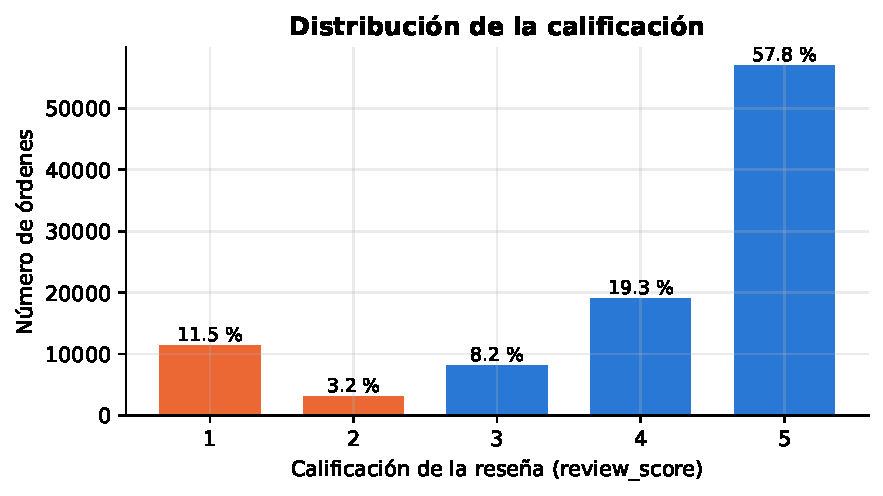
\includegraphics[width=0.9\columnwidth]{dist_review_score}
\caption{Distribución de la calificación de las órdenes. En naranja, las calificaciones agrupadas como insatisfacción.}
\label{fig:score}
\end{figure}


\subsubsection{Datos faltantes e imputación}
Hicimos una revisión de valores nulos y encontramos que solo el 1.92\% de los registros presentaba datos faltantes.
\begin{itemize}
    \item Las variables relacionadas con características del producto (peso, cantidad de fotos, categoría y longitud del nombre) presentaban un 1.4\% de nulos debido a que los vendedores no llenaron esos datos en Olist. Estrategia: Imputamos las variables numéricas usando la mediana y para la categoría creamos una etiqueta nueva llamada ``Desconocido''.
    \item Para la distancia entre comprador y vendedor faltaba el 0.5\% de los datos por códigos postales no mapeados, los cuales también imputamos usando la mediana de las distancias.
    \item Adicionalmente, detectamos un error en 1.343 registros (1.4\%) donde la fecha de entrega a la transportadora aparecía registrada antes de la fecha de aprobación del pago; en estos casos, igualamos esa diferencia de días a cero para evitar tiempos negativos ilógicos. Es importante aclarar que el cálculo de la mediana para la imputación se hará únicamente sobre los datos de entrenamiento para evitar el sesgo o fuga de información.
\end{itemize}

\vspace{1.5em}
\subsubsection{Estrategia de codificación de variables}
Para preparar los datos para los diferentes algoritmos de Machine Learning, definimos las siguientes codificaciones:

\begin{itemize}
    \item Escalado de variables numéricas: Variables como el precio, el peso, el costo del flete y la distancia tienen valores muy dispersos y asimétricos (outliers muy altos). Por esto, primero aplicaremos una transformación logarítmica $\log(1+x)$ y luego las estandarizaremos usando Z-score.
    \item Variables binarias: Las variables lógicas (ej: si el pedido llegó tarde o si comprador y vendedor son del mismo estado) se mantendrán con valores de 0 y 1.
    \item Variables categóricas: Para el método de pago principal usaremos codificación One-Hot Encoding. Para los estados geográficos y las categorías de productos (que son más de 70), seleccionaremos solo las 15 más frecuentes aplicándoles One-Hot Encoding y agruparemos el resto en una categoría llamada ``Otros'' para no aumentar exageradamente la dimensionalidad del modelo.
\end{itemize}



\subsection{Análisis exploratorio}

El factor con mayor correlación empírica con la insatisfacción es el cumplimiento de la promesa de entrega (Fig.~\ref{fig:retraso}). Mientras el pedido llegue dentro de la fecha estimada, la tasa de clientes insatisfechos oscila entre el 9~\% y el 11~\%. En cambio, al acumular cuatro días de retraso, la insatisfacción supera el 60~\%. A nivel global, el 8~\% de las órdenes sufrió retrasos, y dentro de este grupo la insatisfacción trepa al 54,1~\%, frente al 9,2~\% registrado en entregas puntuales. Otro patrón revelador aparece en órdenes que involucran a dos vendedores: la insatisfacción alcanza el 46~\% frente al 12~\% en órdenes de un solo vendedor. Nuestra hipótesis es que estas compras llegan en envíos separados y el cliente califica negativamente al recibir solo una parte del pedido.

\begin{figure}[h!]
\centering
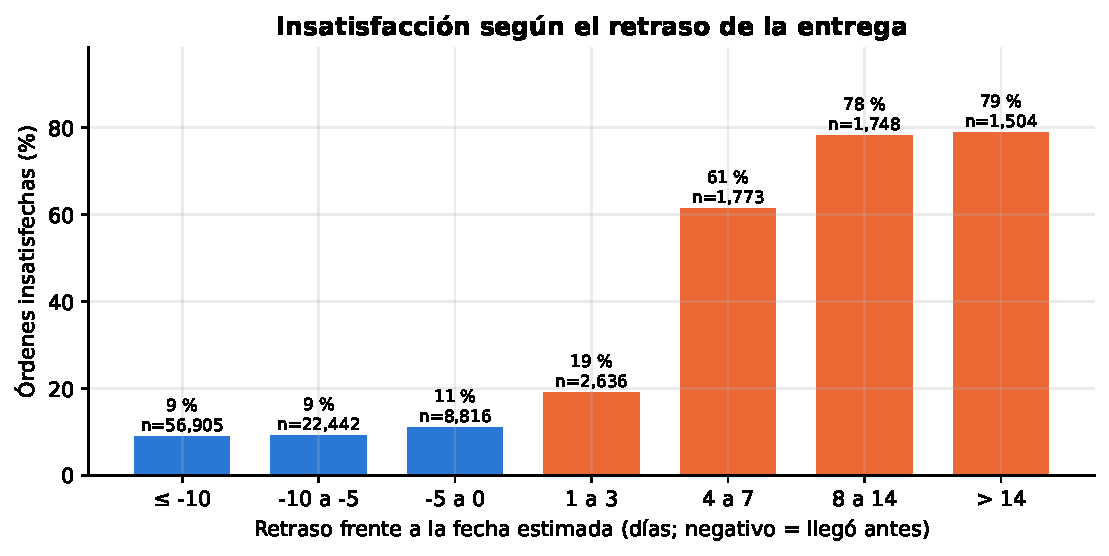
\includegraphics[width=\columnwidth]{insatisfaccion_retraso}
\caption{Porcentaje de órdenes insatisfechas según el retraso de la entrega frente a la fecha estimada. Los valores negativos indican que la orden llegó antes.}
\label{fig:retraso}
\end{figure}

A lo largo del tiempo, la insatisfacción ronda el 10~\% durante casi todo el periodo, pero sube en noviembre de 2017 (16,6~\%), coincidiendo con Black Friday, y en febrero y marzo de 2018 (19,4~\% y 21,2~\%). Son meses de alto volumen de compras donde sospechamos que la logística se congestiona.

Evaluamos también si una mala experiencia en la primera compra castiga la recompra en la plataforma. Contrario a lo esperado, los datos no evidencian un impacto detectable: el 97~\% de los usuarios compra exactamente una vez, y la tasa de recompra entre clientes satisfechos (3,0~\%) y descontentos (2,8~\%) no difiere con significancia estadística ($\chi^2$, $p=0{,}28$). Con un volumen tan bajo de recompras históricas, el conjunto de datos no ofrece base empírica para modelar retención a largo plazo, por lo que este aspecto se mantiene como una premisa de negocio respaldada en un estudio externo~\cite{zeinali2026}.


\vspace{1.5em}
\subsection{Paradigma de aprendizaje y justificación}

Para resolver este problema, hemos decidido estructurar la solución utilizando un paradigma de Clasificación Binaria Supervisada. Las razones que nos llevaron a tomar esta decisión son las siguientes:

\begin{enumerate}
    \item ¿Por qué aprendizaje supervisado? 
    Contamos con una ventaja importante en el conjunto de datos de Olist: tenemos acceso al registro histórico real de las reseñas dejadas por los usuarios. Dado que la etiqueta o ``verdad'' ya existe (sabemos si el cliente quedó contento o no), el enfoque más lógico es el aprendizaje supervisado, ya que el modelo puede aprender directamente de estos ejemplos históricos.
    \vspace{1em}
    \item ¿Por qué clasificación binaria y no regresión o multiclase?
    Aunque la variable original (review\_score) tiene un rango numérico de 1 a 5 estrellas, predecir el número exacto (regresión) o intentar clasificar la orden en una de las 5 categorías exactas (clasificación multiclase) no aporta tanto valor al negocio. Olist necesita alertas tempranas y claras sobre clientes que tuvieron una experiencia muy mala y tienen alto riesgo de abandono. Además, como lo demostraron Wangkiat y Polprasert [6], los modelos multiclase en este escenario tienen un rendimiento muy bajo (con un $F_1$ macro de solo 0.32) porque es difícil diferenciar los matices entre una calificación de 3 y 4 estrellas.
    Por esta razón, nos alineamos con la literatura previa \cite{zeinali2026}, \cite{orman2026}, \cite{zaghloul2024} y definimos el problema de manera binaria: agrupamos las calificaciones 1 y 2 como ``Cliente Insatisfecho'' (clase 1) y las calificaciones de 3 a 5 como ``Cliente Satisfecho'' (clase 0).
    \vspace{1em}
    \item Métricas de evaluación y manejo del desbalance:
    Como vimos en la exploración, nuestros datos están desbalanceados: solo el 12.8\% de las órdenes resultan en insatisfacción. Esto hace que usar la exactitud global (Accuracy) sea engañoso. Si un modelo dice que todos los clientes están satisfechos sin hacer ningún cálculo, tendría un ``éxito'' aparente del 87.2\%, pero sería inútil para la empresa porque fallaría en detectar los verdaderos casos de riesgo. Por eso, en nuestro proyecto evaluaremos el desempeño de los modelos centrándonos en métricas que castiguen los errores en la clase minoritaria (los insatisfechos). Utilizaremos principalmente:
    \begin{enumerate}
        \item Sensibilidad (Recall) y el $F_1$-score de la clase minoritaria para saber cuántos de los clientes realmente insatisfechos logramos detectar.
        \item Área bajo la curva ROC (AUC-ROC) y la exactitud balanceada para medir el rendimiento general del modelo separando bien ambas clases independientemente de cuántos datos haya de cada una.
    \end{enumerate}
    \vspace{1em}
    Finalmente, para tratar el desbalance de los datos durante el entrenamiento de los algoritmos (Entregable II), planeamos probar técnicas como asignarle más peso a los errores en la clase minoritaria o generar datos sintéticos (sobremuestreo), asegurándonos de aplicar esto solo en los pliegues de entrenamiento para que los resultados de validación sigan siendo confiables.
\end{enumerate}


\section{Estado del arte}

El propósito fundamental de esta revisión fue identificar cómo la literatura especializada de Machine Learning ha abordado la predicción de la satisfacción en el comercio electrónico, priorizando aquellos trabajos que utilizaron el mismo conjunto de datos de Olist. Analizamos cuatro artículos resumidos en la Tabla III. Todos los autores abordan el problema bajo el mismo paradigma de clasificación supervisada binaria, agrupando las calificaciones de 1-2 estrellas (insatisfacción) frente a las de 3-5 estrellas. Además, los cuatro estudios coinciden en que la logística y los tiempos de entrega son las características (variables) con mayor capacidad predictiva.

\begin{table*}[!ht]
\centering
\caption{Trabajos previos sobre satisfacción y retención de clientes con los datos de Olist}
\label{tab:sota}
\footnotesize
\begin{tabularx}{\textwidth}{@{}>{\raggedright\arraybackslash}p{2.1cm}>{\raggedright\arraybackslash}p{2.2cm}>{\raggedright\arraybackslash}X>{\raggedright\arraybackslash}p{3.4cm}>{\raggedright\arraybackslash}p{2.8cm}>{\raggedright\arraybackslash}X@{}}
\toprule
Trabajo & Paradigma & Técnicas & Validación & Métricas & Mejor resultado \\
\midrule
Wong y Marikannan~\cite{wong2020} & Supervisado, binario (1--2 vs. 3--5) & Árbol de decisión, RF, red neuronal, SVM; 20 vs. 5 variables; submuestreo, sobremuestreo, SMOTE, ROSE & 50~\% de los datos; partición 70/30; RF con validación cruzada de 1 a 5 pliegues & Exactitud, sensibilidad, especificidad, $F_1$, tiempo & RF: exactitud 87,6~\%, $F_1$ 0,93, especificidad 29,5~\%. El balanceo no mejoró la especificidad \\
\addlinespace
Zaghloul et~al.~\cite{zaghloul2024} & Supervisado, binario (1--2 vs. 3--5) & Regresión logística, SVM, RF, \emph{gradient boosting}, MLP; selección por información mutua; sobremuestreo aleatorio, SMOTE, ADASYN & Partición aleatoria 67/33 por artículo; búsqueda en malla & Exactitud, AUC-ROC, AUC-PR, precisión, sensibilidad y $F_1$ ponderados & RF con sobremuestreo: exactitud 92~\%, $F_1$ ponderado 0,92, AUC-ROC 0,90 \\
\addlinespace
Orman~\cite{orman2026} & Supervisado, binario (1--2 vs. 3--5) & 8 modelos clásicos (RL, NB, árboles, RF, XGBoost, LightGBM, CatBoost) y 5 profundos (CNN, RNN, MLP, GRU-LSTM, LSTM-GRU) & Partición estratificada 80/20; validación cruzada estratificada de 3 pliegues para los clásicos; SMOTE solo en entrenamiento & Exactitud con IC de Wilson, precisión, sensibilidad y $F_1$ por clase, $F_1$ macro y ponderado, exactitud balanceada, MCC, AUC-ROC, AUC-PR & GRU-LSTM: exactitud 86,1~\%, pero sensibilidad de 14,4~\% y $F_1$ de 0,24 en la clase insatisfecha; AUC-ROC 0,56 \\
\addlinespace
Zeinali et~al.~\cite{zeinali2026} & Supervisado, binario (abandono a 180 días), por cliente; K-means para segmentar & K-means sobre RFM; RL, RF, XGBoost con pesos por clase & Partición estratificada 80/20; validación cruzada estratificada de 5 pliegues; variables calculadas antes de la fecha de corte & Exactitud, precisión, sensibilidad, $F_1$, AUC-ROC & XGBoost: exactitud 0,81, $F_1$ 0,81, AUC-ROC 0,85. La calificación promedio es la segunda variable más importante \\
\bottomrule
\end{tabularx}
\end{table*}

\vspace{1em}
Al analizar las técnicas, validación, métricas y resultados de estos trabajos, encontramos dos hallazgos metodológicos clave que adoptaremos para nuestro proyecto:

\begin{enumerate}
    \item El peligro de usar la Exactitud Global (Accuracy): Notamos que varios trabajos reportan exactitudes globales muy altas (entre el 86\% y el 92\%), pero fallan en la detección de la clase que realmente importa: los clientes insatisfechos. Por ejemplo, Wong y Marikannan \cite{wong2020} logran un 87.6\% de exactitud con un Random Forest, pero su modelo solo es capaz de identificar correctamente al 29.5\% de los clientes insatisfechos (especificidad). De manera similar, aunque Zaghloul et al. \cite{zaghloul2024} reportan un 92\% de exactitud general, omiten desglosar el rendimiento específico en la clase minoritaria. Un caso más transparente es el de Orman \cite{orman2026}, quien logró una exactitud del 86.1\% usando redes neuronales híbridas (GRU-LSTM), pero advierte que su modelo solo tiene una sensibilidad (Recall) del 14.4\% para los clientes insatisfechos.
    \vspace{1em}
    \item La definición de la unidad de análisis y la fuga de información Un aprendizaje importante surgió al revisar cómo otros dividían sus datos (metodología de validación). Vimos que Zaghloul et al. \cite{zaghloul2024} hicieron la partición de entrenamiento y prueba (67/33) a nivel de artículo individual. Esto es riesgoso porque los productos que pertenecen a una misma orden (y comparten el mismo tiempo de entrega y calificación) pueden quedar repartidos entre los datos de entrenamiento y los de prueba, generando una grave "fuga de información" (data leakage). Para evitar este error en nuestro proyecto, decidimos usar como unidad de análisis la orden de compra completa y no los artículos individuales.
    \vspace{1em}
    \item Finalmente, el artículo de Zeinali et al. \cite{zeinali2026} fue fundamental para entender el contexto del problema. Ellos desarrollaron un modelo de retención (XGBoost con exactitud de 81\%) e identificaron que el historial de buenas o malas calificaciones es la segunda variable más importante para predecir si un cliente abandonará la plataforma. Esto justifica plenamente la utilidad de nuestro modelo de insatisfacción como paso previo para mejorar la fidelización en Olist.
\end{enumerate}

\vspace{1em}
De igual manera, se identifica aquellas métricas reportadas en la literatura que no fueron abordadas en las clases teóricas del curso. Para un problema con $K$ clases, $n_k$ observaciones en la clase $k$ y un total de $N=\sum_k n_k$ muestras, las variantes macro y ponderada de $F_1$ se definen como:
\begin{equation}
F_1^{\text{macro}} = \frac{1}{K}\sum_{k=1}^{K} F_{1,k}, \qquad F_1^{\text{pond}} = \sum_{k=1}^{K} \frac{n_k}{N} F_{1,k},
\end{equation}
extendiendo la misma ponderación a la precisión y la sensibilidad. Por su parte, el AUC-ROC y el AUC-PR representan las integrales bajo las curvas ROC y de precisión-sensibilidad:
\begin{equation}
\text{AUC-ROC} = \int_0^1 \text{TPR}\; d(\text{FPR}), \qquad \text{AUC-PR} = \int_0^1 P\; dR .
\end{equation}
En términos probabilísticos, el AUC-ROC cuantifica la probabilidad de que el clasificador asigne una puntuación de riesgo mayor a una orden insatisfecha elegida al azar que a una satisfactoria.


\bibliographystyle{IEEEtran}
\bibliography{referencias}

\end{document}
